\documentclass[journal,12pt,twocolumn]{IEEEtran}
\usepackage{setspace}
\usepackage{gensymb}
\usepackage{caption}
%\usepackage{multirow}
%\usepackage{multicolumn}
%\usepackage{subcaption}
%\doublespacing
\singlespacing
\usepackage{csvsimple}
\usepackage{amsmath}
\usepackage{multicol}
%\usepackage{enumerate}
\usepackage{amssymb}
%\usepackage{graphicx}
\usepackage{newfloat}
%\usepackage{syntax}
\usepackage{listings}
\usepackage{iithtlc}
\usepackage{color}
\usepackage{tikz}
\usetikzlibrary{shapes,arrows}



%\usepackage{graphicx}
%\usepackage{amssymb}
%\usepackage{relsize}
%\usepackage[cmex10]{amsmath}
%\usepackage{mathtools}
%\usepackage{amsthm}
%\interdisplaylinepenalty=2500
%\savesymbol{iint}
%\usepackage{txfonts}
%\restoresymbol{TXF}{iint}
%\usepackage{wasysym}
\usepackage{amsthm}
\usepackage{mathrsfs}
\usepackage{txfonts}
\usepackage{stfloats}
\usepackage{cite}
\usepackage{cases}
\usepackage{mathtools}
\usepackage{caption}
\usepackage{enumerate}	
\usepackage{enumitem}
\usepackage{amsmath}
%\usepackage{xtab}
\usepackage{longtable}
\usepackage{multirow}
%\usepackage{algorithm}
%\usepackage{algpseudocode}
\usepackage{enumitem}
\usepackage{mathtools}
\usepackage{hyperref}
%\usepackage[framemethod=tikz]{mdframed}
\usepackage{listings}
    %\usepackage[latin1]{inputenc}                                 %%
    \usepackage{color}                                            %%
    \usepackage{array}                                            %%
    \usepackage{longtable}                                        %%
    \usepackage{calc}                                             %%
    \usepackage{multirow}                                         %%
    \usepackage{hhline}                                           %%
    \usepackage{ifthen}                                           %%
  %optionally (for landscape tables embedded in another document): %%
    \usepackage{lscape}     


\usepackage{url}
\def\UrlBreaks{\do\/\do-}


%\usepackage{stmaryrd}


%\usepackage{wasysym}
%\newcounter{MYtempeqncnt}
\DeclareMathOperator*{\Res}{Res}
%\renewcommand{\baselinestretch}{2}
\renewcommand\thesection{\arabic{section}}
\renewcommand\thesubsection{\thesection.\arabic{subsection}}
\renewcommand\thesubsubsection{\thesubsection.\arabic{subsubsection}}

\renewcommand\thesectiondis{\arabic{section}}
\renewcommand\thesubsectiondis{\thesectiondis.\arabic{subsection}}
\renewcommand\thesubsubsectiondis{\thesubsectiondis.\arabic{subsubsection}}

% correct bad hyphenation here
\hyphenation{op-tical net-works semi-conduc-tor}

%\lstset{
%language=C,
%frame=single, 
%breaklines=true
%}

%\lstset{
	%%basicstyle=\small\ttfamily\bfseries,
	%%numberstyle=\small\ttfamily,
	%language=Octave,
	%backgroundcolor=\color{white},
	%%frame=single,
	%%keywordstyle=\bfseries,
	%%breaklines=true,
	%%showstringspaces=false,
	%%xleftmargin=-10mm,
	%%aboveskip=-1mm,
	%%belowskip=0mm
%}

%\surroundwithmdframed[width=\columnwidth]{lstlisting}
\def\inputGnumericTable{}                                 %%
\lstset{
%language=C,
frame=single, 
breaklines=true,
columns=fullflexible
}
 

\begin{document}
%
\tikzstyle{block} = [rectangle, draw,
    text width=3em, text centered, minimum height=3em]
\tikzstyle{sum} = [draw, circle, node distance=3cm]
\tikzstyle{input} = [coordinate]
\tikzstyle{output} = [coordinate]
\tikzstyle{pinstyle} = [pin edge={to-,thin,black}]

\theoremstyle{definition}
\newtheorem{theorem}{Theorem}[section]
\newtheorem{problem}{Problem}
\newtheorem{proposition}{Proposition}[section]
\newtheorem{lemma}{Lemma}[section]
\newtheorem{corollary}[theorem]{Corollary}
\newtheorem{example}{Example}[section]
\newtheorem{definition}{Definition}[section]
%\newtheorem{algorithm}{Algorithm}[section]
%\newtheorem{cor}{Corollary}
\newcommand{\BEQA}{\begin{eqnarray}}
\newcommand{\EEQA}{\end{eqnarray}}
\newcommand{\define}{\stackrel{\triangle}{=}}

\bibliographystyle{IEEEtran}
%\bibliographystyle{ieeetr}

\providecommand{\nCr}[2]{\,^{#1}C_{#2}} % nCr
\providecommand{\nPr}[2]{\,^{#1}P_{#2}} % nPr
\providecommand{\mbf}{\mathbf}
\providecommand{\pr}[1]{\ensuremath{\Pr\left(#1\right)}}
\providecommand{\qfunc}[1]{\ensuremath{Q\left(#1\right)}}
\providecommand{\sbrak}[1]{\ensuremath{{}\left[#1\right]}}
\providecommand{\lsbrak}[1]{\ensuremath{{}\left[#1\right.}}
\providecommand{\rsbrak}[1]{\ensuremath{{}\left.#1\right]}}
\providecommand{\brak}[1]{\ensuremath{\left(#1\right)}}
\providecommand{\lbrak}[1]{\ensuremath{\left(#1\right.}}
\providecommand{\rbrak}[1]{\ensuremath{\left.#1\right)}}
\providecommand{\cbrak}[1]{\ensuremath{\left\{#1\right\}}}
\providecommand{\lcbrak}[1]{\ensuremath{\left\{#1\right.}}
\providecommand{\rcbrak}[1]{\ensuremath{\left.#1\right\}}}
\theoremstyle{remark}
\newtheorem{rem}{Remark}
\newcommand{\sgn}{\mathop{\mathrm{sgn}}}
\providecommand{\abs}[1]{\left\vert#1\right\vert}
\providecommand{\res}[1]{\Res\displaylimits_{#1}} 
\providecommand{\norm}[1]{\lVert#1\rVert}
\providecommand{\mtx}[1]{\mathbf{#1}}
\providecommand{\mean}[1]{E\left[ #1 \right]}
\providecommand{\fourier}{\overset{\mathcal{F}}{ \rightleftharpoons}}
%\providecommand{\hilbert}{\overset{\mathcal{H}}{ \rightleftharpoons}}
\providecommand{\system}{\overset{\mathcal{H}}{ \longleftrightarrow}}
	%\newcommand{\solution}[2]{\textbf{Solution:}{#1}}
\newcommand{\solution}{\noindent \textbf{Solution: }}
\newcommand{\myvec}[1]{\ensuremath{\begin{pmatrix}#1\end{pmatrix}}}
\providecommand{\dec}[2]{\ensuremath{\overset{#1}{\underset{#2}{\gtrless}}}}
\DeclarePairedDelimiter{\ceil}{\lceil}{\rceil}
%\numberwithin{equation}{subsection}
%\numberwithin{equation}{section}
%\numberwithin{problem}{subsection}
%\numberwithin{definition}{subsection}
\makeatletter
\@addtoreset{figure}{section}
\makeatother

\let\StandardTheFigure\thefigure
%\renewcommand{\thefigure}{\theproblem.\arabic{figure}}
\renewcommand{\thefigure}{\thesection}


%\numberwithin{figure}{subsection}

%\numberwithin{equation}{subsection}
%\numberwithin{equation}{section}
%\numberwithin{equation}{problem}
%\numberwithin{problem}{subsection}
\numberwithin{problem}{section}
%%\numberwithin{definition}{subsection}
%\makeatletter
%\@addtoreset{figure}{problem}
%\makeatother
\makeatletter
\@addtoreset{table}{section}
\makeatother

\let\StandardTheFigure\thefigure
\let\StandardTheTable\thetable
\let\vec\mathbf
%%\renewcommand{\thefigure}{\theproblem.\arabic{figure}}
%\renewcommand{\thefigure}{\theproblem}

%%\numberwithin{figure}{section}

%%\numberwithin{figure}{subsection}



\def\putbox#1#2#3{\makebox[0in][l]{\makebox[#1][l]{}\raisebox{\baselineskip}[0in][0in]{\raisebox{#2}[0in][0in]{#3}}}}
     \def\rightbox#1{\makebox[0in][r]{#1}}
     \def\centbox#1{\makebox[0in]{#1}}
     \def\topbox#1{\raisebox{-\baselineskip}[0in][0in]{#1}}
     \def\midbox#1{\raisebox{-0.5\baselineskip}[0in][0in]{#1}}

\vspace{3cm}

\title{ 
	\logo{
Python with Linear Algebra: 2D 
	}
}

\author{ G V V Sharma$^{*}$% <-this % stops a space
	\thanks{*The author is with the Department
		of Electrical Engineering, Indian Institute of Technology, Hyderabad
		502285 India e-mail:  gadepall@iith.ac.in. All content in this manual is released under GNU GPL.  Free and open source.}
	
}	

\maketitle

\tableofcontents

\bigskip

\renewcommand{\thefigure}{\theenumi}
\renewcommand{\thetable}{\theenumi}

\begin{abstract}
This manual introduces matrix computations using python and the properties of a triangle.
\end{abstract}
\section{Line}
\begin{enumerate}[label=\thesection.\arabic*
,ref=\thesection.\theenumi]
\item
\label{prob:draw_triangle}
Let
\begin{equation}
\vec{A} =
\begin{pmatrix}
-2
\\
-2
\end{pmatrix},
\vec{B} =
\begin{pmatrix}
1
\\
3
\end{pmatrix},
\vec{C} =
\begin{pmatrix*}[r]
4
\\
-1
\end{pmatrix*}.
\end{equation}
Draw $\Delta ABC$.
\\
\solution
The following code yields the desired plot in Fig. \ref{fig:triangle_def}
\lstinputlisting{./codes/draw_triangle.py}
\begin{figure}
\centering
\includegraphics[width=\columnwidth]{./figs/triangle.eps}
\caption{}
\label{fig:triangle_def}
\end{figure}
%
\item
%
Find the equation of $AB$.
\\
\solution  The desired equation is obtained as
\begin{align}
\label{eq:line_dir}
AB: \quad \vec{x} &= \vec{A}+ \lambda_1 \brak{\vec{B}-\vec{A}}
\\
&= -\myvec{2\\2}+ \lambda_1\myvec{3\\5}
\end{align}
%
\item Find the direction vector and the normal vector for $AB$
\\
\solution Let
\begin{align}
T_{AB} = \myvec{\vec{A} & \vec{B}} = \myvec{-2 & 1\\ -2 & 3}
\end{align}
The direction vector of $AB$ is 
\begin{equation}
\label{eq:dir_vec}
\vec{m} = \vec{B}-\vec{A} = T_{AB} \myvec{-1 \\ 1} = \myvec{3\\5}
\end{equation}
%
The normal vector $\vec{n}$ is defined as
\begin{align}
\label{eq:line_nor}
\vec{n}^T\vec{m} &= 0
\\
\implies \vec{n}&= \myvec{0 & 1 \\ -1 & 0}\vec{m} = \myvec{5\\-3}
\end{align}
%
\item Write a python code for computing the direction and normal vectors. 
%
\solution 
Save the following code  as \textbf{coeffs.py} and execute.
\label{prob:line_eq}
\lstinputlisting{./codes/coeffs.py}

\item Find the equation of the line in terms of the normal 
vector.
\\
\solution The desired equation is
\begin{align}
\label{eq:line_norm}
\vec{n}^T\brak{\vec{x} - \vec{A}}=\vec{n}^T\brak{\vec{x} - \vec{B}}&= 0
\\
\implies \myvec{5&-3}\vec{x} = -\myvec{5&-3}\myvec{2\\2} &= -4
\end{align}
%
\item
%
Find the equations of $BC$ and $CA$.
\end{enumerate}
\section{Altitudes of a Triangle}
\begin{enumerate}[label=\thesection.\arabic*
,ref=\thesection.\theenumi]
\item
In $\Delta ABC$,  Let $\vec{P}$ be a point on $BC$ such that $AP \perp BC$.  Then $AP$ is defined to be 
an {\em altitude} of $\Delta ABC$.

\item
\label{prob:alt_eq}
Find the equation of $AP$.
\\
\solution The normal vector of $AP$ is $\vec{B} - \vec{C}$. From 
\eqref{eq:line_norm}, the equation of $AP$ is
\begin{align}
\label{eq:alt_ap}
\brak{\vec{B} - \vec{C}}^T\brak{\vec{x} - \vec{A}}&= 0
\\
\implies \myvec{-3&4}\vec{x} = -\myvec{-3&4}\myvec{2\\2} &= -2
\end{align}

%\lstinputlisting{./codes/alt_eq.py}
%
\item Find the equation of the altitude $BQ$.
\\
\solution The desired equation is 
\begin{align}
\label{eq:alt_bq}
\brak{\vec{C} - \vec{A}}^T\brak{\vec{x} - \vec{B}}&= 0
\\
\implies \myvec{6&1}\vec{x} = \myvec{6&1}\myvec{1\\3} &= 9
\end{align}
\item Find the equation of the altitude $CR$.
%
\item Find the point of intersection of $AP$ and $BQ$.
\solution \eqref{eq:alt_ap} and \eqref{eq:alt_bq} can be stacked together into the matrix equation
\begin{align}
\label{eq:alt_mat}
 \myvec{-3&4 \\ 6&1}\vec{x} = \myvec{-2\\9}
\end{align}
The following code computes the point of intersection.
\begin{lstlisting}
https://raw.githubusercontent.com/gadepall/school/master/linalg/2D/python_2d/codes/orthocentre.py
\end{lstlisting}

\item Find the point of intersection of  and $BQ$ and $CR$. Comment.
\item Find $\vec{P}$
%
\\
\solution The following code finds the required points.
\begin{lstlisting}
https://raw.githubusercontent.com/gadepall/school/master/linalg/2D/python_2d/codes/alt_foot.py
\end{lstlisting}
\item Find $\vec{Q}$ and $\vec{R}$.
\item Draw $AP, BQ$ and $CR$ and verify that they meet at a point 
$\vec{H}$.  
\\
\solution 
\begin{lstlisting}
https://raw.githubusercontent.com/gadepall/school/master/linalg/2D/python_2d/codes/alt_draw.py
\end{lstlisting}

\end{enumerate}

\section{Medians of a Triangle}
\begin{enumerate}[label=\thesection.\arabic*
,ref=\thesection.\theenumi]

\item
Find the coordinates of $D, E$ and $F$ of the mid points of $AB, BC$ and $CA$ respectively for  $\Delta ABC$. 
\\ 
\solution
The coordinates of the mid points are given by
%
\begin{align}
D &= \frac{B+C}{2}, E = \frac{C+A}{2}, F = \frac{A+B}{2}
\end{align}
%
The following code computes the values resulting in
\begin{equation}
D = \begin{pmatrix}
2.5
\\
1
\end{pmatrix},
E = \begin{pmatrix}
1
\\
-1.5
\end{pmatrix},
F = \begin{pmatrix}
-0.5
\\
0.5
\end{pmatrix},
\end{equation}
\lstinputlisting{./codes/mid_points.py}
\item
Find the equations of $AD,BE$ and $CF$. These lines are the {\em medians} of $\Delta ABC$
\\
\solution Use the code in Problem \ref{prob:line_eq}. 
%
\item
\label{prob:median}
Find the point of intersection of $AD$ and $CF$.
\\
\solution
Let the respective equations  be
\begin{align}
\vec{n}_1^T\vec{x} &= p_1 \text{ and}
\\
\vec{n}_2^T\vec{x} &= p_2
\end{align}
This can be written as the matrix equation
\begin{align}
\myvec{ \vec{n}_1^T
\\
\vec{n}_2^T}
\vec{x}
&=
\vec{p}
\\
\implies N^T \vec{x}
&=
\vec{p}
\end{align}
%
where
\begin{equation}
N = \myvec{ \vec{n}_1 &
\vec{n}_2},
\end{equation}
%
The point of intersection is then obtained as
\begin{align}
\vec{x} &= \brak{N^T}^{-1}  \vec{p}
\\
&= N^{-T} \vec{p}
\end{align}
%
The following code yields the point of intersection 
\begin{equation}
\vec{G} =
\begin{pmatrix}
1
\\
0
\end{pmatrix}
\end{equation}
\lstinputlisting{./codes/line_intersect.py}
\item
Using the code in Problem \ref{prob:median}, verify that $\vec{G}$ is the point of intersection of $BE,CF$ as 
well as
$AD,BE$.  $\vec{G}$ is known as the {\em centroid} of $\Delta ABC$.
\\
\item
Graphically show that the medians of $\Delta ABC$ meet at the centroid.
\\
\item
Verify that
\begin{equation}
G = \frac{A+B+C}{3}
\end{equation}
\end{enumerate}
\section{Angle Bisectors of a Triangle}
%
\begin{enumerate}[label=\thesection.\arabic*
,ref=\thesection.\theenumi]

\item
In $\Delta ABC$, let $U$ be a point on $BC$ such that $\angle BAU = \angle CAU$. Then $AU$ is known as the {\em angle bisector}.

\item
Find the length of $AB,BC$ and $CA$
\\
\solution The length of $CA$ is given by
\begin{align}
CA = \norm{\vec{C}-\vec{A}}
%&= \sqrt{37}.
\end{align}
The following code calculates the respective values as
%
\begin{equation}
AB =  5.83, BC =  5, CA =  6.08
\end{equation}
%
\lstinputlisting{./codes/side_length.py}
\item
If $AU,BV$ and $CW$ are the angle bisectors, find the coordinates of $\vec{U},\vec{V}$ and $\vec{W}$.
\\
\solution Using the section formula,
\begin{align}
\vec{W} &= \frac{AW.\vec{B}+WB.\vec{A}}{AW + WB} = \frac{\frac{AW}{WB}.\vec{B}+\vec{A}}{\frac{AW}{WB} + 1}
\\
&= \frac{\frac{CA}{BC}.\vec{B}+\vec{A}}{\frac{CA}{BC} + 1}
\\
&= \frac{{CA}\times \vec{B}+{BC}\times \vec{A}}{{BC} + {CA}}
\\
&= \frac{a\times \vec{A} + b\times \vec{B}}{a + b}
\end{align}
where $a = BC, b = CA$, 
since the angle bisector has the property that
%
\begin{equation}
\frac{AW}{WB} = \frac{CA}{AB}
\end{equation}
%
\item Write a program to find $\vec{U},\vec{V},\vec{W}$.
%
%\lstinputlisting{./codes/angle_bisect_coord.py}
\item
Find the intersection of $AU$ and $BV$.% and $CW$ and verify that they meet at a point $I$.  
\\
\solution Using the code in Problem \ref{prob:median}, the desired point of intersection is
\begin{equation}
\vec{I} = 
\begin{pmatrix}
1.15
\\
0.14
\end{pmatrix}
\end{equation}
%
It is easy to verify that even $BV$ and $CW$ meet at the same point.  $\vec{I}$ is known as
the {\em incentre} of $\Delta ABC$. 
\item
Draw $AU, BV$ and $CW$ and verify that they meet at a point $\vec{I}$.  
%%
\item
Verify that
\begin{align}
\vec{I} = \frac{BC.\vec{A} + CA.\vec{B} + AB.\vec{C}}{AB+BC+CA}
\end{align}
%
\\
\item
\label{prob:incircle_normal}
Let the perpendicular from $\vec{I}$ to $AB$ be $IX$. If the equation of $AB$ is
%
\begin{align}
\vec{n}^T\brak{\vec{x}-\vec{A}} = 0
\end{align}
%
show that
\begin{align}
IX = \frac{\abs{\vec{n}^T\brak{\vec{I}-\vec{A}}}}{\norm{\vec{n}}}
\end{align}
%
Verify through a Python script.
\item If $IY \perp BC$ and $IZ \perp CA$,
verify that
\begin{equation}
IX = IY = IZ = r
\end{equation}
$r$ is known as the {\em inradius} of $\Delta ABC$.
%\lstinputlisting{./codes/inradius.py}
\item Draw the incircle of $\triangle ABC$
\item Draw the circumcircle of $\triangle ABC$

\end{enumerate}
\end{document}


